\documentclass[]{article}
\usepackage{lmodern}
\usepackage{amssymb,amsmath}
\usepackage{ifxetex,ifluatex}
\usepackage{fixltx2e} % provides \textsubscript
\ifnum 0\ifxetex 1\fi\ifluatex 1\fi=0 % if pdftex
  \usepackage[T1]{fontenc}
  \usepackage[utf8]{inputenc}
\else % if luatex or xelatex
  \ifxetex
    \usepackage{mathspec}
  \else
    \usepackage{fontspec}
  \fi
  \defaultfontfeatures{Ligatures=TeX,Scale=MatchLowercase}
\fi
% use upquote if available, for straight quotes in verbatim environments
\IfFileExists{upquote.sty}{\usepackage{upquote}}{}
% use microtype if available
\IfFileExists{microtype.sty}{%
\usepackage{microtype}
\UseMicrotypeSet[protrusion]{basicmath} % disable protrusion for tt fonts
}{}
\usepackage[margin=1in]{geometry}
\usepackage{hyperref}
\hypersetup{unicode=true,
            pdfborder={0 0 0},
            breaklinks=true}
\urlstyle{same}  % don't use monospace font for urls
\usepackage{color}
\usepackage{fancyvrb}
\newcommand{\VerbBar}{|}
\newcommand{\VERB}{\Verb[commandchars=\\\{\}]}
\DefineVerbatimEnvironment{Highlighting}{Verbatim}{commandchars=\\\{\}}
% Add ',fontsize=\small' for more characters per line
\usepackage{framed}
\definecolor{shadecolor}{RGB}{248,248,248}
\newenvironment{Shaded}{\begin{snugshade}}{\end{snugshade}}
\newcommand{\KeywordTok}[1]{\textcolor[rgb]{0.13,0.29,0.53}{\textbf{#1}}}
\newcommand{\DataTypeTok}[1]{\textcolor[rgb]{0.13,0.29,0.53}{#1}}
\newcommand{\DecValTok}[1]{\textcolor[rgb]{0.00,0.00,0.81}{#1}}
\newcommand{\BaseNTok}[1]{\textcolor[rgb]{0.00,0.00,0.81}{#1}}
\newcommand{\FloatTok}[1]{\textcolor[rgb]{0.00,0.00,0.81}{#1}}
\newcommand{\ConstantTok}[1]{\textcolor[rgb]{0.00,0.00,0.00}{#1}}
\newcommand{\CharTok}[1]{\textcolor[rgb]{0.31,0.60,0.02}{#1}}
\newcommand{\SpecialCharTok}[1]{\textcolor[rgb]{0.00,0.00,0.00}{#1}}
\newcommand{\StringTok}[1]{\textcolor[rgb]{0.31,0.60,0.02}{#1}}
\newcommand{\VerbatimStringTok}[1]{\textcolor[rgb]{0.31,0.60,0.02}{#1}}
\newcommand{\SpecialStringTok}[1]{\textcolor[rgb]{0.31,0.60,0.02}{#1}}
\newcommand{\ImportTok}[1]{#1}
\newcommand{\CommentTok}[1]{\textcolor[rgb]{0.56,0.35,0.01}{\textit{#1}}}
\newcommand{\DocumentationTok}[1]{\textcolor[rgb]{0.56,0.35,0.01}{\textbf{\textit{#1}}}}
\newcommand{\AnnotationTok}[1]{\textcolor[rgb]{0.56,0.35,0.01}{\textbf{\textit{#1}}}}
\newcommand{\CommentVarTok}[1]{\textcolor[rgb]{0.56,0.35,0.01}{\textbf{\textit{#1}}}}
\newcommand{\OtherTok}[1]{\textcolor[rgb]{0.56,0.35,0.01}{#1}}
\newcommand{\FunctionTok}[1]{\textcolor[rgb]{0.00,0.00,0.00}{#1}}
\newcommand{\VariableTok}[1]{\textcolor[rgb]{0.00,0.00,0.00}{#1}}
\newcommand{\ControlFlowTok}[1]{\textcolor[rgb]{0.13,0.29,0.53}{\textbf{#1}}}
\newcommand{\OperatorTok}[1]{\textcolor[rgb]{0.81,0.36,0.00}{\textbf{#1}}}
\newcommand{\BuiltInTok}[1]{#1}
\newcommand{\ExtensionTok}[1]{#1}
\newcommand{\PreprocessorTok}[1]{\textcolor[rgb]{0.56,0.35,0.01}{\textit{#1}}}
\newcommand{\AttributeTok}[1]{\textcolor[rgb]{0.77,0.63,0.00}{#1}}
\newcommand{\RegionMarkerTok}[1]{#1}
\newcommand{\InformationTok}[1]{\textcolor[rgb]{0.56,0.35,0.01}{\textbf{\textit{#1}}}}
\newcommand{\WarningTok}[1]{\textcolor[rgb]{0.56,0.35,0.01}{\textbf{\textit{#1}}}}
\newcommand{\AlertTok}[1]{\textcolor[rgb]{0.94,0.16,0.16}{#1}}
\newcommand{\ErrorTok}[1]{\textcolor[rgb]{0.64,0.00,0.00}{\textbf{#1}}}
\newcommand{\NormalTok}[1]{#1}
\usepackage{graphicx,grffile}
\makeatletter
\def\maxwidth{\ifdim\Gin@nat@width>\linewidth\linewidth\else\Gin@nat@width\fi}
\def\maxheight{\ifdim\Gin@nat@height>\textheight\textheight\else\Gin@nat@height\fi}
\makeatother
% Scale images if necessary, so that they will not overflow the page
% margins by default, and it is still possible to overwrite the defaults
% using explicit options in \includegraphics[width, height, ...]{}
\setkeys{Gin}{width=\maxwidth,height=\maxheight,keepaspectratio}
\IfFileExists{parskip.sty}{%
\usepackage{parskip}
}{% else
\setlength{\parindent}{0pt}
\setlength{\parskip}{6pt plus 2pt minus 1pt}
}
\setlength{\emergencystretch}{3em}  % prevent overfull lines
\providecommand{\tightlist}{%
  \setlength{\itemsep}{0pt}\setlength{\parskip}{0pt}}
\setcounter{secnumdepth}{0}
% Redefines (sub)paragraphs to behave more like sections
\ifx\paragraph\undefined\else
\let\oldparagraph\paragraph
\renewcommand{\paragraph}[1]{\oldparagraph{#1}\mbox{}}
\fi
\ifx\subparagraph\undefined\else
\let\oldsubparagraph\subparagraph
\renewcommand{\subparagraph}[1]{\oldsubparagraph{#1}\mbox{}}
\fi

%%% Use protect on footnotes to avoid problems with footnotes in titles
\let\rmarkdownfootnote\footnote%
\def\footnote{\protect\rmarkdownfootnote}

%%% Change title format to be more compact
\usepackage{titling}

% Create subtitle command for use in maketitle
\newcommand{\subtitle}[1]{
  \posttitle{
    \begin{center}\large#1\end{center}
    }
}

\setlength{\droptitle}{-2em}
  \title{}
  \pretitle{\vspace{\droptitle}}
  \posttitle{}
  \author{}
  \preauthor{}\postauthor{}
  \date{}
  \predate{}\postdate{}


\begin{document}

\subsubsection{Load library}\label{load-library}

\begin{Shaded}
\begin{Highlighting}[]
\KeywordTok{library}\NormalTok{(tidyverse)}
\KeywordTok{library}\NormalTok{(Hmisc)}
\end{Highlighting}
\end{Shaded}

\subsubsection{Read in data}\label{read-in-data}

\begin{Shaded}
\begin{Highlighting}[]
\KeywordTok{library}\NormalTok{(readxl)}
\KeywordTok{setwd}\NormalTok{(}\StringTok{"../Week06"}\NormalTok{)}
\NormalTok{fname <-}\StringTok{ "week6_coffee_chains.xlsx"}
\KeywordTok{excel_sheets}\NormalTok{(fname)}
\end{Highlighting}
\end{Shaded}

\begin{verbatim}
## [1] "starbucks" "timhorton" "dunkin"
\end{verbatim}

\begin{Shaded}
\begin{Highlighting}[]
\NormalTok{dfStar <-}\StringTok{ }\KeywordTok{read_excel}\NormalTok{(fname, }\DecValTok{1}\NormalTok{)}
\NormalTok{dfTimh <-}\StringTok{ }\KeywordTok{read_excel}\NormalTok{(fname, }\DecValTok{2}\NormalTok{)}
\NormalTok{dfDunk <-}\StringTok{ }\KeywordTok{read_excel}\NormalTok{(fname, }\DecValTok{3}\NormalTok{)}
\end{Highlighting}
\end{Shaded}

\subsubsection{Fifty States}\label{fifty-states}

\begin{Shaded}
\begin{Highlighting}[]
\KeywordTok{library}\NormalTok{(albersusa)}
\NormalTok{us      <-}\StringTok{ }\KeywordTok{usa_composite}\NormalTok{()}
\NormalTok{us_map  <-}\StringTok{ }\NormalTok{broom}\OperatorTok{::}\KeywordTok{tidy}\NormalTok{(us, }\DataTypeTok{region =} \StringTok{"name"}\NormalTok{)}

\KeywordTok{library}\NormalTok{(usmap)}
\end{Highlighting}
\end{Shaded}

\begin{verbatim}
## Warning: package 'usmap' was built under R version 3.3.3
\end{verbatim}

\begin{Shaded}
\begin{Highlighting}[]
\KeywordTok{data}\NormalTok{(statepop)}

\NormalTok{StarUS <-}\StringTok{ }\NormalTok{dfStar }\OperatorTok\StringTok{ }
\StringTok{  }\KeywordTok{filter}\NormalTok{(Country }\OperatorTok{==}\StringTok{ "US"}\NormalTok{) }\OperatorTok\StringTok{ }
\StringTok{  }\KeywordTok{mutate}\NormalTok{(}\DataTypeTok{state =}\NormalTok{ openintro}\OperatorTok{::}\KeywordTok{abbr2state}\NormalTok{(}\StringTok{`}\DataTypeTok{State/Province}\StringTok{`}\NormalTok{))}
\end{Highlighting}
\end{Shaded}

\begin{verbatim}
## Warning: package 'bindrcpp' was built under R version 3.3.3
\end{verbatim}

\begin{Shaded}
\begin{Highlighting}[]
\NormalTok{avgStarUS <-}\StringTok{ }\NormalTok{StarUS }\OperatorTok\StringTok{ }
\StringTok{  }\KeywordTok{group_by}\NormalTok{(state) }\OperatorTok\StringTok{ }
\StringTok{  }\KeywordTok{summarise}\NormalTok{(}\DataTypeTok{count =} \KeywordTok{n}\NormalTok{(), }\DataTypeTok{ST =} \KeywordTok{unique}\NormalTok{(}\StringTok{`}\DataTypeTok{State/Province}\StringTok{`}\NormalTok{)) }\OperatorTok\StringTok{ }
\StringTok{  }\KeywordTok{left_join}\NormalTok{(statepop, }\DataTypeTok{by =} \KeywordTok{c}\NormalTok{(}\StringTok{"ST"}\NormalTok{ =}\StringTok{ "abbr"}\NormalTok{)) }\OperatorTok\StringTok{ }
\StringTok{  }\KeywordTok{mutate}\NormalTok{(}\DataTypeTok{Avg =}\NormalTok{ count}\OperatorTok{/}\NormalTok{pop_}\DecValTok{2015} \OperatorTok{*}\StringTok{ }\FloatTok{1e5}\NormalTok{) }


\NormalTok{p <-}\StringTok{ }\KeywordTok{ggplot}\NormalTok{() }\OperatorTok{+}
\StringTok{  }\KeywordTok{geom_map}\NormalTok{(}\DataTypeTok{data =}\NormalTok{ avgStarUS, }\KeywordTok{aes}\NormalTok{(}\DataTypeTok{fill =}\NormalTok{ Avg, }\DataTypeTok{map_id =}\NormalTok{ state),}
           \DataTypeTok{color=}\StringTok{"white"}\NormalTok{, }\DataTypeTok{size =} \FloatTok{0.01}\NormalTok{, }\DataTypeTok{map =}\NormalTok{ us_map) }\OperatorTok{+}\StringTok{ }
\StringTok{  }\KeywordTok{scale_fill_distiller}\NormalTok{(}\DataTypeTok{name =} \StringTok{"Number"}\NormalTok{, }\DataTypeTok{palette =} \StringTok{"Spectral"}\NormalTok{) }\OperatorTok{+}
\StringTok{  }\KeywordTok{expand_limits}\NormalTok{(}\DataTypeTok{x =}\NormalTok{ us_map}\OperatorTok{$}\NormalTok{long, }\DataTypeTok{y =}\NormalTok{ us_map}\OperatorTok{$}\NormalTok{lat) }\OperatorTok{+}
\StringTok{  }\KeywordTok{coord_map}\NormalTok{() }\OperatorTok{+}
\StringTok{  }\KeywordTok{theme_void}\NormalTok{() }\OperatorTok{+}
\StringTok{  }\KeywordTok{theme}\NormalTok{(}\DataTypeTok{legend.position=}\KeywordTok{c}\NormalTok{(.}\DecValTok{88}\NormalTok{, .}\DecValTok{4}\NormalTok{))}\OperatorTok{+}
\StringTok{  }\KeywordTok{ggtitle}\NormalTok{( }\StringTok{"Starbucks Stores per 100, 000 population"}\NormalTok{ ) }\OperatorTok{+}
\StringTok{  }\KeywordTok{labs}\NormalTok{(}\DataTypeTok{caption =} \StringTok{"Source: US Census Demogrpahic Data 2015"}\NormalTok{)}
\NormalTok{p}
\end{Highlighting}
\end{Shaded}

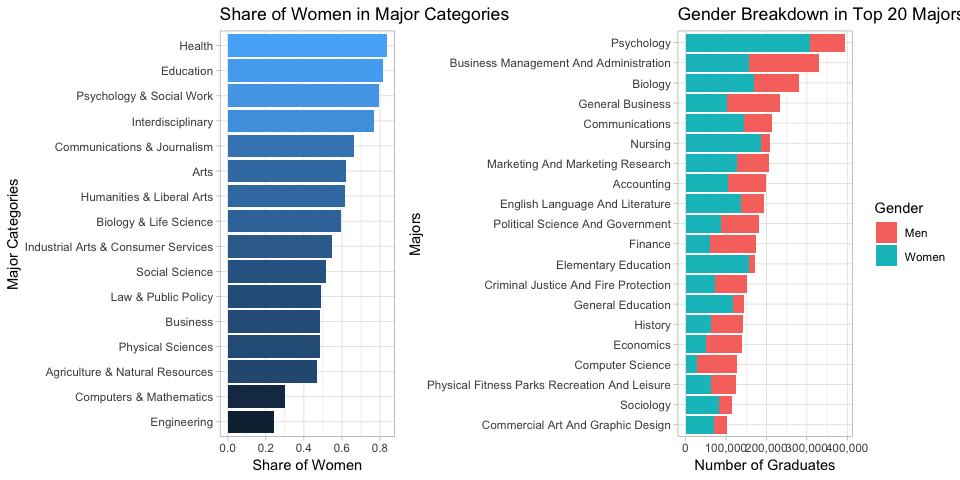
\includegraphics{Week06_files/figure-latex/unnamed-chunk-3-1.pdf}

\begin{Shaded}
\begin{Highlighting}[]
\CommentTok{#p + coord_map("polyconic")}
\end{Highlighting}
\end{Shaded}

\subsubsection{Dot Density Map for
CONUS}\label{dot-density-map-for-conus}

\begin{Shaded}
\begin{Highlighting}[]
\NormalTok{StarCONUS <-}\StringTok{ }\KeywordTok{filter}\NormalTok{(StarUS, }\StringTok{`}\DataTypeTok{State/Province}\StringTok{`} \OperatorTok{!=}\StringTok{ "HI"} \OperatorTok{&}\StringTok{ `}\DataTypeTok{State/Province}\StringTok{`} \OperatorTok{!=}\StringTok{ "AK"}\NormalTok{)}
\NormalTok{avgStarCONUS <-}\StringTok{ }\KeywordTok{filter}\NormalTok{(avgStarUS, ST }\OperatorTok{!=}\StringTok{ "HI"} \OperatorTok{&}\StringTok{ }\NormalTok{ST }\OperatorTok{!=}\StringTok{ "AK"}\NormalTok{)}
 
\NormalTok{t <-}\StringTok{ }\KeywordTok{ggplot}\NormalTok{() }\OperatorTok{+}
\StringTok{  }\KeywordTok{geom_map}\NormalTok{(}\DataTypeTok{data =}\NormalTok{ avgStarCONUS, }\KeywordTok{aes}\NormalTok{(}\DataTypeTok{fill =}\NormalTok{ Avg, }\DataTypeTok{map_id =}\NormalTok{ state),}
           \DataTypeTok{color=}\StringTok{"white"}\NormalTok{, }\DataTypeTok{size =} \FloatTok{0.01}\NormalTok{, }\DataTypeTok{map =}\NormalTok{ us_map) }\OperatorTok{+}\StringTok{ }
\StringTok{  }\KeywordTok{scale_fill_distiller}\NormalTok{(}\DataTypeTok{name =} \StringTok{"Number"}\NormalTok{, }\DataTypeTok{palette =} \StringTok{"Spectral"}\NormalTok{) }\OperatorTok{+}
\StringTok{  }\KeywordTok{geom_point}\NormalTok{(}\DataTypeTok{data =}\NormalTok{ StarCONUS, }\KeywordTok{aes}\NormalTok{(}\DataTypeTok{x =}\NormalTok{ Longitude, }\DataTypeTok{y =}\NormalTok{ Latitude), }\DataTypeTok{size =} \FloatTok{0.04}\NormalTok{, }\DataTypeTok{alpha =} \FloatTok{0.1}\NormalTok{) }\OperatorTok{+}

\StringTok{  }\KeywordTok{expand_limits}\NormalTok{(}\DataTypeTok{x =}\NormalTok{ us_map}\OperatorTok{$}\NormalTok{long, }\DataTypeTok{y =}\NormalTok{ us_map}\OperatorTok{$}\NormalTok{lat) }\OperatorTok{+}
\StringTok{  }\KeywordTok{coord_map}\NormalTok{() }\OperatorTok{+}
\StringTok{  }\KeywordTok{theme_void}\NormalTok{() }\OperatorTok{+}
\StringTok{  }\KeywordTok{theme}\NormalTok{(}\DataTypeTok{legend.position=}\KeywordTok{c}\NormalTok{(.}\DecValTok{88}\NormalTok{, .}\DecValTok{4}\NormalTok{))}\OperatorTok{+}
\StringTok{  }\KeywordTok{ggtitle}\NormalTok{( }\StringTok{"Starbucks Stores per 100, 000 population"}\NormalTok{ ) }\OperatorTok{+}
\StringTok{  }\KeywordTok{labs}\NormalTok{(}\DataTypeTok{caption =} \StringTok{"Source: US Census Demogrpahic Data 2015"}\NormalTok{)}
\NormalTok{t}
\end{Highlighting}
\end{Shaded}

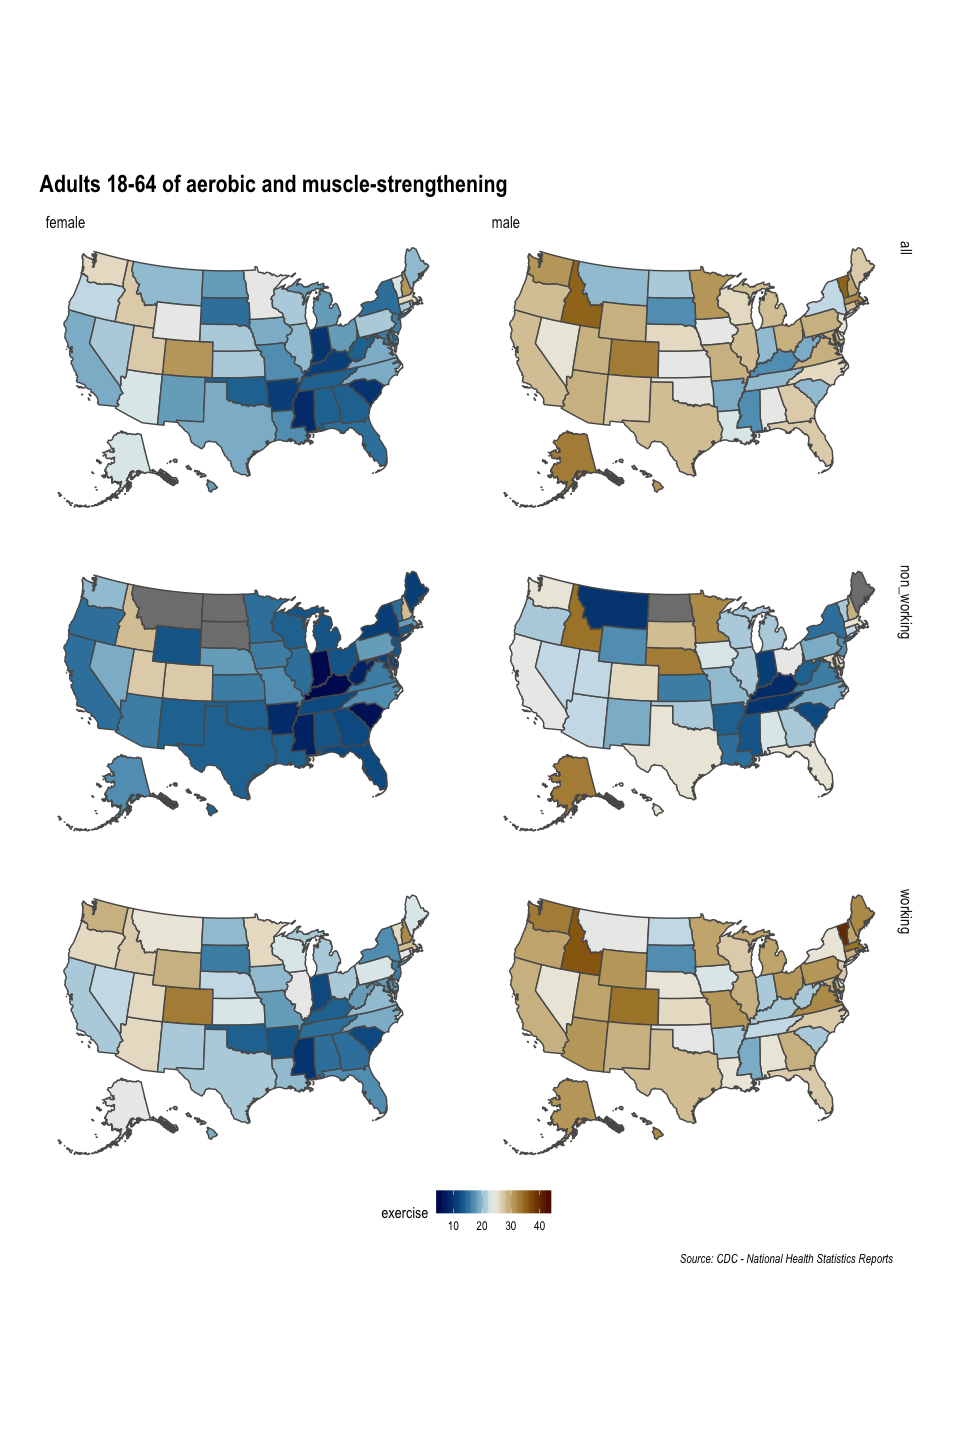
\includegraphics{Week06_files/figure-latex/unnamed-chunk-4-1.pdf}

\begin{Shaded}
\begin{Highlighting}[]
\CommentTok{#t + coord_map("polyconic")}
\end{Highlighting}
\end{Shaded}


\end{document}
